
\subsection{Reif- und Eisbildung}
\label{subsec:Reifbildung}

Liegt die Oberflächentemperatur auf dem Wärmeübertrager des Verdampfers nicht nur unter dem Taupunktpunkt der feuchten Luft, sondern auch unter dem Gefrierpunkt, kann es zum Gefrieren der kondensierten Tropfen und/oder zur Desublimation von Wasserpartikeln auf der Oberfläche kommen. Dieser Abschnitt soll einen Überblick über diese zwei thermodynamischen Phänome geben. Da in dieser Arbeit nicht der Reifbildungsprozess im Hauptfokus steht, sondern  der technische Aspekt der Abtauung, wird der Eisbildungsprozess hier nur kurz erläutert.

In der Literatur gibt es zahlreiche Quellen, die sich mit der Reif- bzw. Eisbildung auseinander setzen. Die Quellen beschreiben den Kristallbildungsprozess sowohl aus der rein theoretischer Sicht als auch mittels simulationsrelevanten und technischen Überlegungen bzw. Untersuchungen. Der scheinbar triviale Prozess der Bildung eines Eiskristalles auf einer Oberfläche und sein weiteres Wachstumsverhalten ist sehr komplex und Gegenstand zahlreicher aktueller und schon abgeschlossener Forschungsprojekte.

Neben den theoretischen Grundlagen wird in der Arbeit von \textsc{\citeauthor{Schydlo2010}} ein Simulationsmodell für den Reifbildungs- und Abtauprozess auf einem Rohr entwickelt. Zudem sind bisherige Arbeiten zu der Thematik in \citep{Schydlo2010} aufgelistet und zusammengefasst. 
Praktische Untersuchungen sowie Versuchsaufbauten zum Thema der Vereisung von Luftkühlern werden in \textsc{\citeauthor{Sahinagic2004}} und \textsc{\citeauthor{Kosowski2009}} beschrieben. In den Arbeiten werden die Vereisungs- und innovative Abtauungsprozesse von einer CO$_2$-Wärmepumpe, die zur Heizung von Passivhäuser eingesetzt wird, untersucht.   



Es gibt zahlreiche Einflussgrößen, die auf den Prozess und die Form des Eiskristalls und späteren Reif einwirkten. 
  Die wichtigsten Einflussgrößen sind die Luftgeschwindigkeit, die Lufttemperatur, die Luftfeuchte, die Oberflächentemperatur und die Zeit. Um den Reif charakterisieren zu können, werden folgende Größen zur Hilfe genommen: die Reifdicke, die Reifdichte, die Porösität und die Wärmeleitfähigkeit. 

In der Arbeit von \textsc{\citeauthor{Hayashi1977}} aus dem Jahre 1977 wird der Eiskristallwachstum in drei Phasen unterteilt:

\begin{enumerate}
\item Eindimensionales Kristallwachstum
\item Reifschichtwachstumsphase 
\item Vergletscherung.
\end{enumerate}


\begin{figure}[htb]
\centering		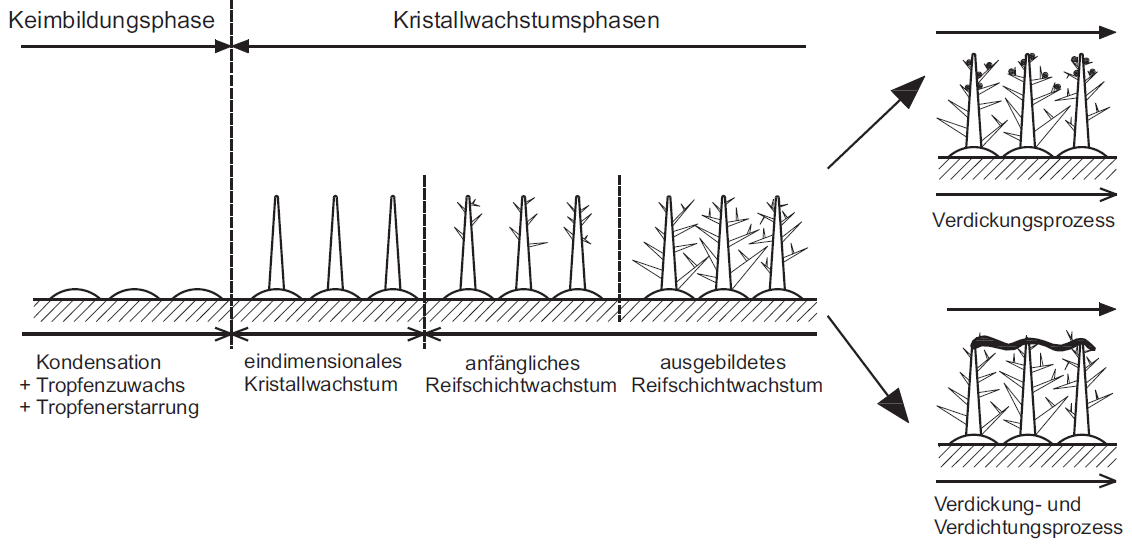
\includegraphics[width=0.85\textwidth]{Pictures/Reifbildungsphasen_Schydlo.png}
\caption{Kristallwachstum auf einer ebenen Oberfläche \citep{Schydlo2010}}
\label{fig:Kristallwachstum}
\end{figure}


In Abbildung \ref{fig:Kristallwachstum} sind die drei Kristallwachstums-Phasen nach \textsc{\citeauthor{Hayashi1977}} sowie die vorhergehende Keimbildungsphase, eingeführt in \citep{Sahinagic2004}, dargestellt. 

\subsubsection*{Keimbildungsphase}

In der Keimbildungsphase bilden sich zunächst Wassertropfen auf der Lamellenoberfläche, die trotz Temperaturen kleiner als der Gefrierpunkt nicht erstarren, sondern zu größeren Tropfen anwachsen. Je kleiner die Unterkühlung, desto größer werden die Tropfen, bevor sie erstarren und in die erste Kristallwachstumsphase übergehen. 

\subsubsection*{Eindimensionales Kristallwachstum}
Die erste Phase ist gekennzeichnet durch Kristallwachstum senkrecht zur Oberfläche und mit einheitlicher Wachstumsgeschwindigkeit. Dies führt aufgrund der sich stetig vermehrenden Kristalle zu einer erhöhten Rauigkeit.  

\subsubsection*{Reifschichtwachstumsphase}
In der zweiten Phase beginnt das dreidimensionale Wachstum. Die Kristalle fangen an sich miteinander zu verästeln. Ein poröses Kristallgitter entsteht. Aufgrund des  Wärmeleitwiderstandes, der mit der Reifdicke steigt, erhöht sich die Oberflächentemperatur der Reifschicht. Des weiteren kommt es zu einem Massenstrom innerhalb der Reifschicht, ausgelöst durch Diffusion. Die Diffusion rührt aus  dem  Konzentrationsunterschieden zwischen der Lamelle und der Reifoberfläche. Der Wassermassenstrom läuft in das poröse Kristallgitter und gefriert dort in Nähe der Lamelle. Die Dichte der Reifschicht steigt und mit ihr der Wärmewiderstand. Dies führt zu einer Erhöhung der Oberflächentemperatur der Reifschicht und schließlich zur Überschreitung des Gefrierpunktes von Eis. Die Spitzen des Kristalle schmelzen und es bildet sich Kondensat. Die dritte Wachstumsphase beginnt. 

\subsubsection*{Vergletscherung}

Das flüssige Wasser läuft aufgrund der Kapillarwirkung der Kristalle in die Zwischenräume des Kristallgitters und gefriert dort wieder. Die Kristallgitter werden dichter und kompakter. Dies führt zur Steigerung der Wärmeleitfähigkeit der Reifschicht. Es wird von einer Vergletscherung gesprochen. Die Oberflächentemperatur der Reifschicht sinkt erneut und fällt erneut unter den Gefrierpunkt. Nun kann die feuchte Luft erneut an der Oberfläche des Reifs desublimieren. Der Prozess wiederholt sich solange, bis das Eis so kompakt ist, dass kein weiteres Kondensat mehr in die Reifschicht eindringen kann. 

\subsection*{Physikalische Eigenschaften von Eiskristallen}

 Im vorangegangenen Abschnitt \ref{subsec:Reifbildung} wurden die einzelnen Bildungsphasen von Eiskristallen beschrieben. In diesem Abschnitt wird auf die Eigenschaften von Eiskristallen eingegangen und dargestellt wie sie sich während eines Vereisungsvorganges eines Luftkühlers verändern. 
 
Gefriert ein Tropfen Wasser und wird zum Eiskristall, so verändern sich die physikalischen Eigenschaften des Tropfens. In der Arbeit von \textsc{\citeauthor{Schydlo2010}} verdeutlichen zunächst zwei Diagramme, abgebildet in \ref{fig:Zeitverlaufe von Reifdichte und -dicke}, wie sich die Reifdicke und die Reifdichte während eines Vereisungsvorgang verändern. 

\begin{figure}
\centering
    \subfigure[Reifdichte]
    {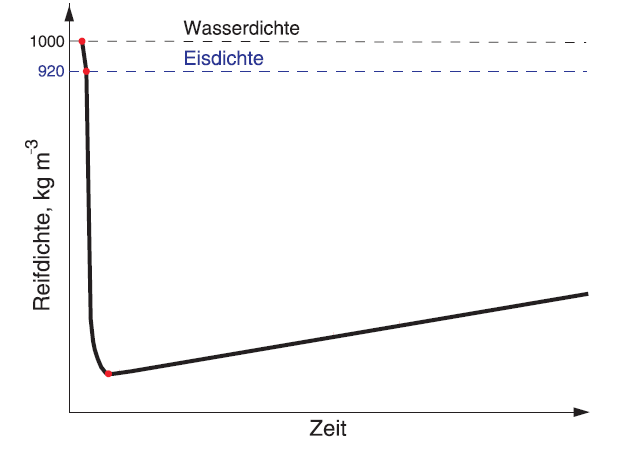
\includegraphics[width=0.50\textwidth]{Pictures/Reifdichte_Schydlo.png}}
    \subfigure[Reifdicke]{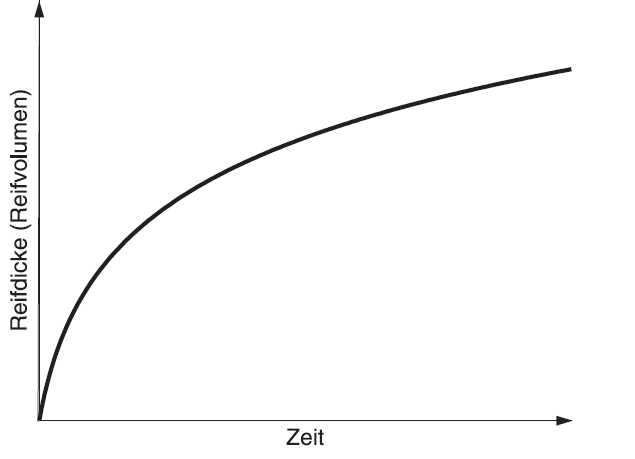
\includegraphics[width=0.48\textwidth]{Pictures/Reifdicke_Schydlo.png}}
\caption{Schematischer Reifdichte- und Reifdickeverläufe beim Vereisungsvorgang eines Tropfen Wassers \cite{Schydlo2010}}
\label{fig:Zeitverlaufe von Reifdichte und -dicke}
\end{figure}

Da Diagramm \ref{fig:Zeitverlaufe von Reifdichte und -dicke}(a) zeigt den Dichteverlauf, aufgetragen über die Vereisungszeit. Die Dichte eines Tropfens fällt beim Gefrieren von 1000 kg/m$^3$ auf 920 kg/m$^3$ sinkt. Danach tritt das in Abschnitt \ref{subsec:Reifbildung} beschriebene eindimensionale Wachstum ein, sodass die Reifdichte bis auf ein Minimum fällt. Danach tritt die dreidimensionale Wachstumsphase und dann die Vergletscherungsphase ein. Die Dichte  steigt jetzt langsam, aber kontinuierlich wieder an.

\begin{figure}[htb]
\centering	
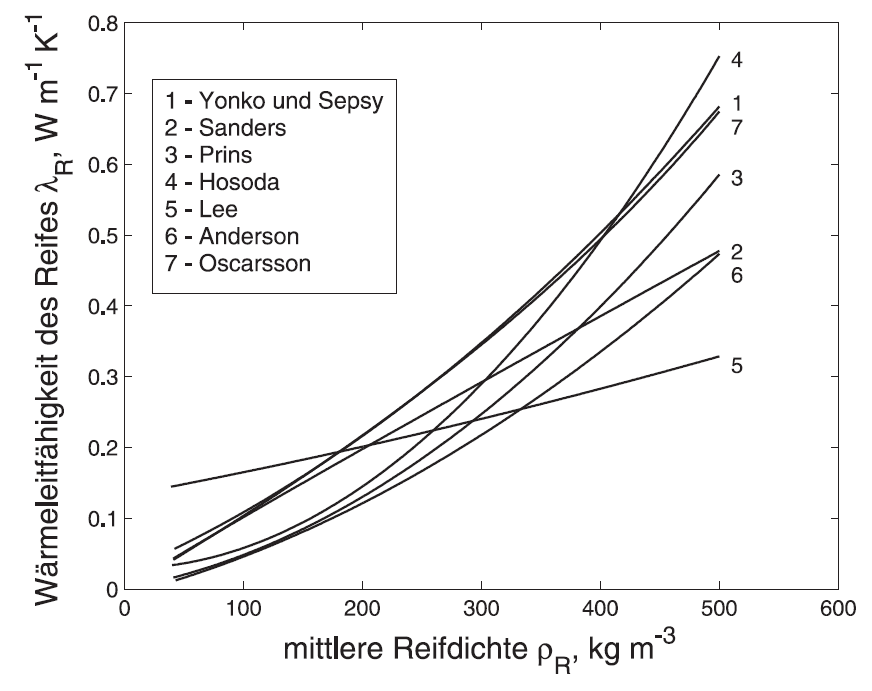
\includegraphics[width=0.55\textwidth]{Pictures/Waermeleitfaehigkeit_Schydlo.png}
\caption{Wärmeleitfähigkeit des Reifs aufgetragen über die mittlere Reifdichte \citep{Schydlo2010}}
\label{fig:Waermeleitfaehigkeit}
\end{figure}

Im \ref{fig:Zeitverlaufe von Reifdichte und -dicke}(b) ist der Reifdickenverlauf aufgetragen. Aus diesem lässt sich entnehmen, dass kurz nach Beginn die zeitliche Änderung der Reifdicke maximal ist. Das heißt, dass der Massenstrom an Kondensat, das sich an der Lamelle absondert und dann gefriert, am Anfang am größten ist und findet während des eindimensionalen Wachstums auf statt. Beim dreidimensionalen Wachstum und späteren Vergletscherung flacht die Kurve ab und strebt gegen einen Sättigungswert. 


 
Mit der Reifdicke verändert sich wiederum die Wärmeleitfähigkeit des Reifes, abgebildet in \ref{fig:Waermeleitfaehigkeit}. In dem Diagramm sind mehrere Berechnungsmodelle aufgetragen, die die Wärmeleitfähigkeit als Funktion der mittleren Reifdichte abbilden. Alle Modelle sagen einen Anstieg von $\lambda$ mit steigender Reifdichte voraus. Dies hängt mit der Verdichtung des Eises während der Vergletscherungsphase zusammen. Die führt dazu, dass Reif mit einer geringen Dichte gleichzeitig als sehr guter Isolator fungiert. \citep{Baehr2013}  \citep{Kosowski2009}


